\hypertarget{contributor-location}{%
\subsubsection{Contributor Location}\label{contributor-location}}

Question: What is the location of contributors?

\hypertarget{description}{%
\paragraph{Description}\label{description}}

Geographical location from which contributors contribute, where they
live, or where they work.

\hypertarget{objectives}{%
\paragraph{Objectives}\label{objectives}}

To determine global locations of contributors in an effort to understand
work practices and times zones. To identify where contributions do not
come from in an effort to improve engagement in these areas.

\hypertarget{implementation}{%
\paragraph{Implementation}\label{implementation}}

\hypertarget{filters}{%
\subparagraph{Filters}\label{filters}}

Filter contributions by:

\begin{itemize}
\tightlist
\item
  \textbf{Location.} Attempt to group locations in regions to have
  multiple levels of reporting. Location is a purposely ambiguous term
  in this context, and could refer to region, country, state, locale, or
  time zone.
\item
  \textbf{Period of time.} Start and finish date of the period. Default:
  forever. Period during which contributions are counted.
\item
  \textbf{Type of contributor}, for example:

  \begin{itemize}
  \tightlist
  \item
    Repository authors
  \item
    Issue authors
  \item
    Code review participants
  \item
    Mailing list authors
  \item
    Event participants
  \item
    IRC authors
  \item
    Blog authors
  \item
    By release cycle
  \item
    Programming languages of the project
  \item
    Role or function in project
  \end{itemize}
\end{itemize}

\hypertarget{visualizations}{%
\subparagraph{Visualizations}\label{visualizations}}

Dot Density Map:

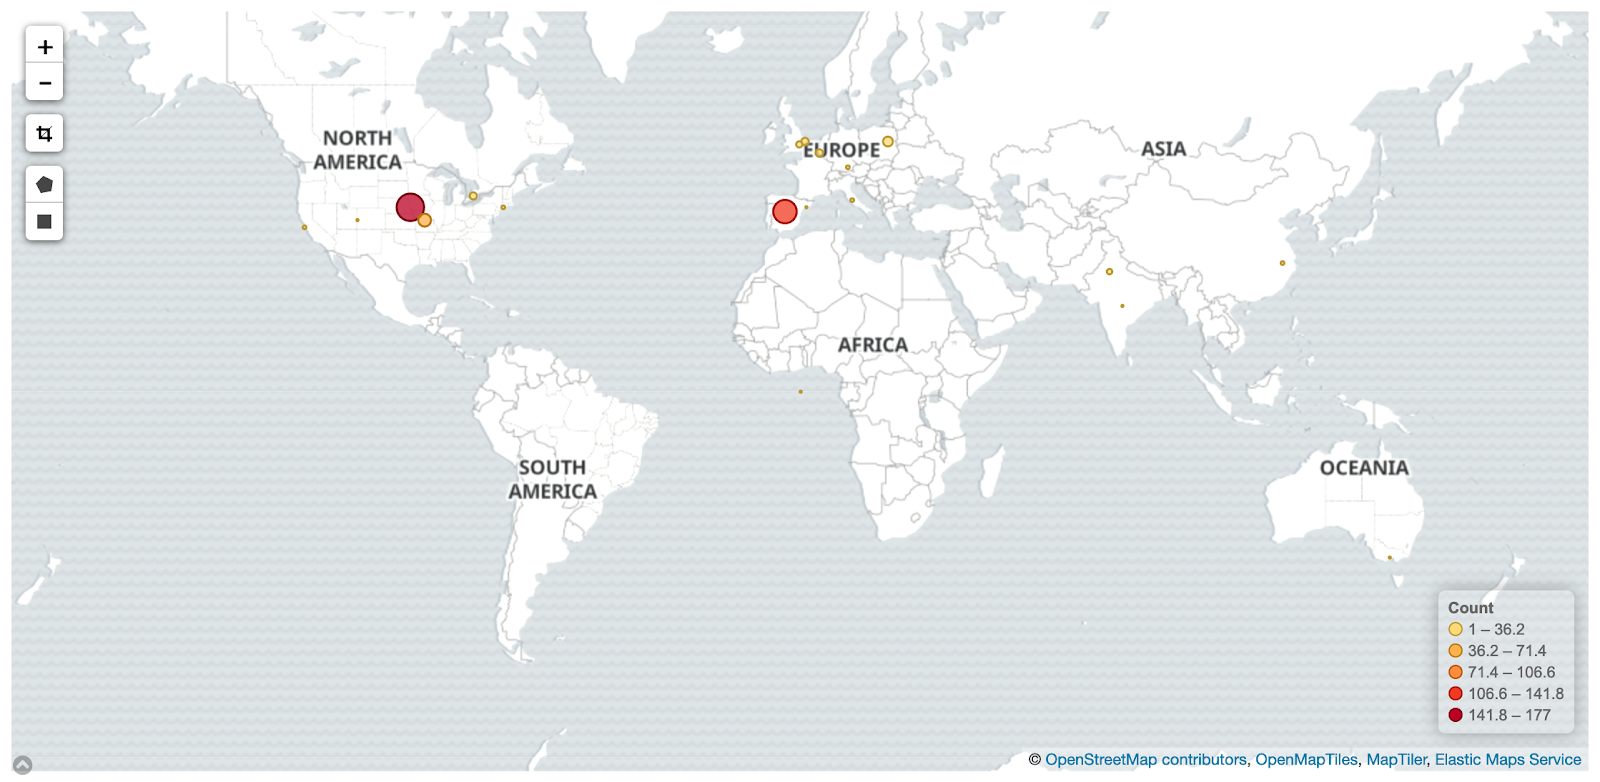
\includegraphics{images/contributor-location_dot-density-map.png}

Source:
\href{https://chaoss.biterg.io/goto/a62f3584a41c1c4c1af5d04b9809a860}{\url{https://chaoss.biterg.io/goto/a62f3584a41c1c4c1af5d04b9809a860}}

Visual heat map:

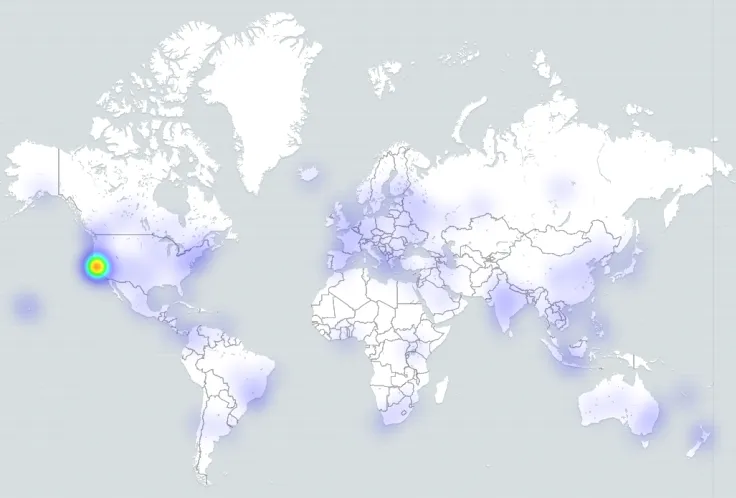
\includegraphics{images/contributor-location_heatmap.png}

Source:
\href{https://blog.bitergia.com/2018/11/20/ubers-community-software-development-analytics-for-open-source-offices}{\url{https://blog.bitergia.com/2018/11/20/ubers-community-software-development-analytics-for-open-source-offices}}

\hypertarget{tools-providing-the-metric}{%
\subparagraph{Tools providing the
metric}\label{tools-providing-the-metric}}

\begin{itemize}
\tightlist
\item
  GrimoireLab
\item
  Augur
\end{itemize}

\hypertarget{data-collection-strategies}{%
\subparagraph{Data Collection
Strategies}\label{data-collection-strategies}}

Different approaches can be used to collect information about location:

\begin{itemize}
\tightlist
\item
  Collect the location information from a contributor's profile in the
  system of engagement.
\item
  Use IP address geolocation of the most frequent locations that
  contributions are made.
\item
  Infer geographical location from the timestamp in contributions.
\item
  Survey contributors.
\end{itemize}

The key challenge for collecting data is determining the location of the
contributor. Best practice would be to leverage any profile information
available from the system of engagement, and if that is not available
then use IP geolocation to determine the most frequent location of
contribution from that individual. Note that contributors may enter in
their profile information false or nonsensical location information
(e.g., ``Earth'' or ``Internet''). Note that IP geolocation can provide
large numbers of false positives due to use of VPNs or other IP masking
tools.

An additional consideration would be the use of external data collection
tools such as community surveys or event registration data that could
cross reference systems of engagement profiles. Contributor location
data could be collected inline with event
\href{https://chaoss.community/metric-attendee-demographics/}{attendee
demographics} and
\href{https://chaoss.community/metric-speaker-demographics/}{speaker
demographics}.

\hypertarget{references}{%
\paragraph{References}\label{references}}

\begin{itemize}
\tightlist
\item
  Gonzalez-Barahona, J. M., Robles, G., Andradas-Izquierdo, R., \&
  Ghosh, R. A. (2008). Geographic origin of libre software developers.
  \emph{Information Economics and Policy}, \emph{20}(4), 356-363.
\end{itemize}
